\documentclass[asi]{picINSA}

\usepackage{lmodern}
\usepackage{amsmath}
\usepackage{amssymb}
\usepackage{mathrsfs}


% Bout de code pour enlever le ``chapitre'' écrit à chaque fois
\makeatletter
\def\@makechapterhead#1{
  {\parindent \z@ \raggedright \normalfont
    \interlinepenalty\@M
    \Huge\bfseries  \thechapter.\quad #1\par\nobreak
    \vskip 40\p@
  }}
\makeatother
% Enlève les doubles pages blanches inutiles
\let\cleardoublepage\clearpage



\begin{document}
  \titreGeneral{Rapport}
  \sousTitreGeneral{\newline Sujet RPG 1}
  \titreAcronyme{\LARGE IHME}
  \version{1.00}
  \referenceVersion{bibliographie}

  \couverture{}

  \tableofcontents{}

\chapter{Introduction}
L'objectif de ce projet est, de réaliser un générateur de scénarios pour RPG, et de mettre en place le déroulement de ce scénario. Les différents joueurs pourront être soit humains, soit virtuels. La trame du jeu pourra faire l'objet de re-planiffication si nécessaire, en fonction des actions effectuées par les différents joueurs. L'interface serait très légère de manière à se concentrer sur le scénario et sur le comportement des joueurs virtuels. \\

Dans ce rapport, nous allons commencer par vous présenter les spécifications que nous avons établies à partir de cet énoncé, et dans un second temps la conception à lequelle nous sommes parvenus.


\chapter{Spécifications}
Après réunions et discussions entre les membres du groupe, voici les spécifications auquelles nous sommes parvenues : \\
~\\
\textbf{A faire nécessairement} :
\begin{itemize}
\item Positionnement (PNJ/Objet), méthode de déplacement, gestion de l'inventaire et de l'argent
\item Interaction entre et avec les PNJ (communication)
\item Objectifs/Scénarios/Quête (décomposées en plusieurs étapes, cachées ou explicites)
\item Maître du Jeu (aide du joueur et re-planification du scénario)
\end{itemize}
~\\
\textbf{A faire dans un second temps} :
\begin{itemize}
\item PNJ ayant leurs objectifs et leurs désirs propres
\item Gestion des connaissances (en fonction de l’intelligence)
\item Gestion des distances pour les interactions
\item Lien avec le programme developpé par Quentin BATEUX
\end{itemize}
~\\
\textbf{A faire si possible} :
\begin{itemize}
\item Interaction entre PNJ (communication de l'émotion)
\item Expérience
\item Interaction entre PNJ et path finding et combat (en lien avec ce que fait l'autre groupe RPG)
\end{itemize}
~\\
\textbf{Optionnel} :
\begin{itemize}
\item Interaction évoluées entre PNJ (accointance, amitié, mariage, couple, enfant)
\item Transmission des gènes et des désirs
\item Évolution des objectifs selon des formules de psychologie (formule parabolique de la motivation sur [0;1])
\item Gestion des connaissances "instantanées" sur le monde.
\item Gestion de la respiration
\item Gestion des différents milieux
\item Gestion de la faim et de la soif
\item Gestion des bâtiments
\item Gestion du statut social
\item Tri des objectifs selon la pyramide de Maslow
\end{itemize}


\chapter{Conception}
Nos choix de conception ont été faits en nous basant sur les résultats des synthèses bibliographiques que nous avons faites par groupe de 2. \newline

Une des synthèses concernait l'Intelligence Artificielle dans les jeux vidéos, et après renseignements, nous sommes arrivés à la conclusion que l'utilisation d'un BDI est la solution la plus adaptée au projet. Nous avons donc mis en place un BDI, en l'adaptant à notre projet. \\

L'autre synthèse bibliographique concernait la scénarisation automatique. Nous avons choisi de mettre en place un HTC pour modéliser les actions des personnages. \\

Les fichiers correspondants se trouvent dans le répertoire de developpement fourni avec ce rapport. Le choix du langage s'est porté sur java, dans l'optique d'un éventuel regroupement avec le programme de Quentin BATEUX, développé en java. 


\section{Conception générale}

\subsection{Diagramme de package}
\begin{figure}[!ht]
  \begin{center}
    \includegraphics[width=1\textwidth]{../conception/packages.pdf}
    \caption{Diagramme de packages}	
  \end{center}
\end{figure}

\newpage

\subsection{Diagramme de classe}
Voici le diagramme de classe tel que nous l'avoins imaginé lors de la phase de conception. Il a été complété par la suite d'autres classes, et notre choix s'est finalement porté sur un developpement en anglais, ce qui fait que les noms des classes sont en fait une traduction de celles présentées par ce diagramme.
\begin{figure}[!ht]
  \begin{center}
    \includegraphics[width=1\textwidth]{../conception/Conception.pdf}
    \caption{Diagramme de classe}	
  \end{center}
\end{figure}





\chapter{Implémentation}

\section{PNJ}

Nous avons choisi d'implémenter les PNJ grâce a des threads. Nos PNJ sont donc des automates BDI. Étant donné qu'il parcourt le monde d'eux même il nous ont permis de débuguer le logiciel sans faire de tests unitaires étant donné que les PNJ parcourait le monde et le testait sans que nous agissions. \\

Les PNJ possèdents des caractéristiques. Pour l'instant les PNJ possèdent un sexe, un état et une inteligence mais nous pourrions ajouter facilement d'autre caractéristiques (Force, charisme, sagesse, emotivité, perception auditive, etc.).

\subsection{Désirs}

Nous avons implémenté les désirs et les beliefs des PNJ en utilisant un Verbe reliant une entité et un object. Par exemple une entité et une Position pour un belief correspond à la localisation d'une entité. Pour un désir cela correspond à une entité qui doit se trouver à une position pour que l'entité ayant le désir soit satisfaite. Ce système modulaire permet d'ajouter facilement des données sémantiques dans le programme. Pour l'instant les deux verbes implémentés sont "OWN" et "LEARN", mais il serait très facile d'ajouter des désirs comme "KILL"; "LOOT", "FALLINLOVE" voir "BECOMESUCESSFUL" dans une future version du logiciel.

\section{Gestion des entités du monde}

Nous avons créé un database manager qui pourra être facilement relié à une base de donnée réélle par la suite. Nous utilisons beaucoup l'introspection pour enregistrer les différentes classes du logiciel.

\section{Interface graphique}
Etant donné la taille du projet, nous avons opté pour une interface graphique simple, fonctionnant en ligne de commande. Nous avons mis en place un affichage du monde par \textit{AsciiArt}, complété eventuellement par d'autres informations écrites. La récupération des actions de l'utilisateur se fait par saisi de mots-clés parmis une liste d'actions possibles.

\subsection{Représentation du monde}
La représentation du monde en \textit{AsciiArt} fonctionne ainsi :
\begin{itemize}
\item chaque case du monde est représenté par un carré de 3 lignes et 3 colonnes, soit 9 symboles.
\item 4 types de terrains sont possibles : herbe, terre, forêt, et montagne. Ils sont représentés par les symboles suivants : \\
\begin{tabular}{| c c c | c c c | c c c | c c c | }
 \hline		
  \multicolumn{3}{|c|}{herbe} & \multicolumn{3}{|c|}{terre} & \multicolumn{3}{|c|}{forêt} & \multicolumn{3}{|c|}{montagne} \\	
\hline
    \verb+"+ & \verb+"+ & \verb+"+ & $\equiv$ & $\equiv$ & $\equiv$ & $\phi$ & $\phi$ & $\phi$ & $\triangle$ & $\triangle$ & $\triangle$ \\
    \verb+"+ & \verb+"+ & \verb+"+ & $\equiv$ & $\equiv$ & $\equiv$ & $\phi$ & $\phi$ & $\phi$ & $\triangle$ & $\triangle$ & $\triangle$ \\
    \verb+"+ & \verb+"+ & \verb+"+ & $\equiv$ & $\equiv$ & $\equiv$ & $\phi$ & $\phi$ & $\phi$ & $\triangle$ & $\triangle$ & $\triangle$ \\
 \hline  
 \end{tabular}
~\\
\item un objet est représenté par un $\blacklozenge$ à droite de la case.
\item un PNJ est représenté par un $\theta$ à gauche de la case.
\item le joueur est représenté par un $\bigoplus$ au centre de la case.
\end{itemize}
\subsubsection{Exemple}
Dans l'exemple ci-dessous, on peut voir la représentaion d'une partie de la carte d'un monde. Cette représentation est de 10 cases sur 20, et est centrée sur le joueur. On peut voir,le joueur situé sur la case (50, 50) et des objets dans les différentes cases autour de lui.

\begin{figure}[!ht]
  \begin{center}
    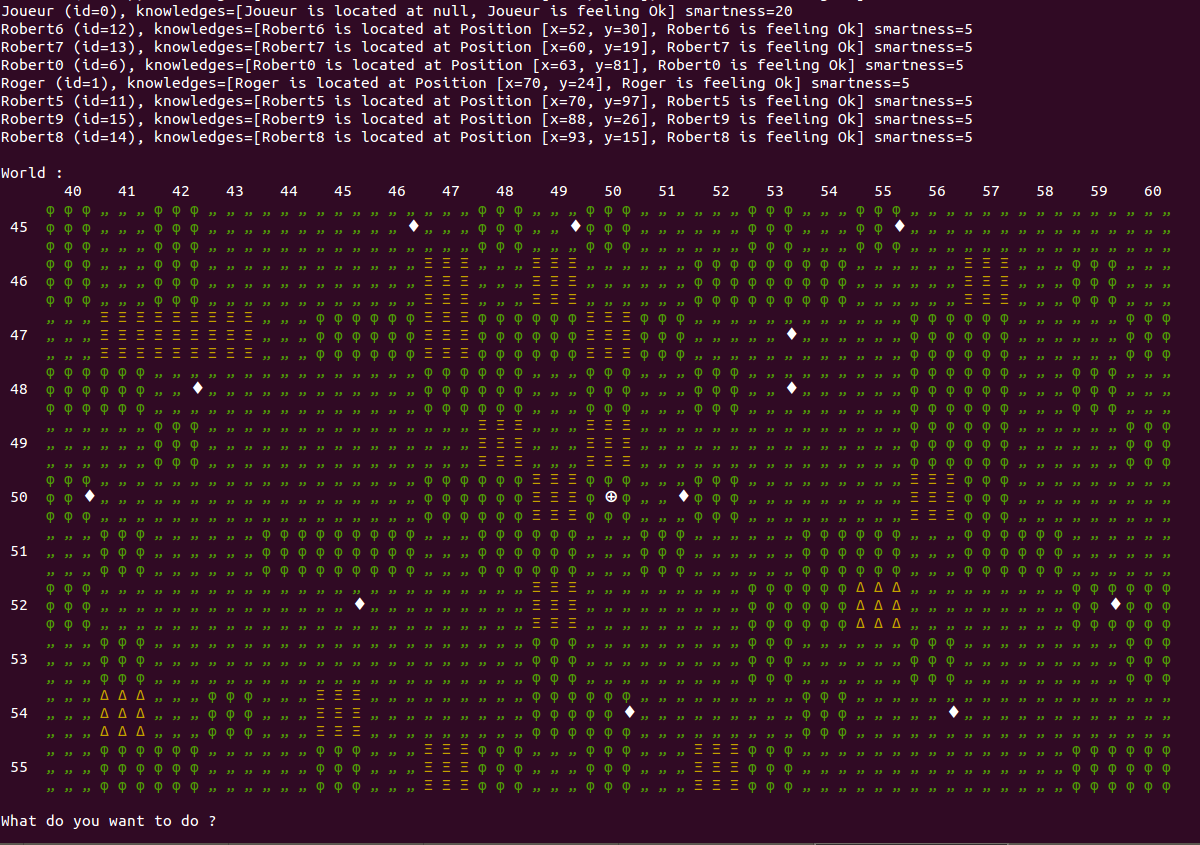
\includegraphics[width=1\textwidth]{images/screenshootWorld01.png}
    \caption{Exemple de la représentation d'un monde (extrait de la carte de taill 10 x 20)}	
  \end{center}
\end{figure}
 On peut voir également au dessus de la carte, quelques indications écrites, qui ne peuvent être représentées graphiquement, comme par exemple le nom des PNJ.
\subsection{Interaction du joueur}
Les interactions avec le joueur se font en lui proposant différentes actions et en le laissant choisir par mot-clés, comme dans l'exemple ci-dessous : \\
\begin{figure}[!ht]
  \begin{center}
    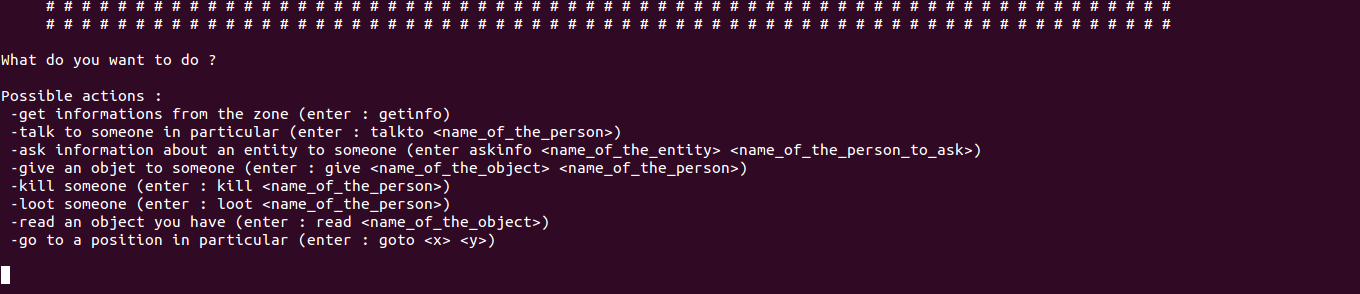
\includegraphics[width=1\textwidth]{images/screenshootUI01.png}
    \caption{Exemple d'action possibles}	
  \end{center}
\end{figure}

Si le joueur rentre autre chose qu'un des mot-clés prévus, cela provoque un message d'erreur. Les  execeptions et erreurs sont reportées à l'utilisateur. \\

Le jeu est actuellement en anglais, mais tous les messages d'interaction avec le joueur sont implémentés dans le code sous forme de constantes de façon à rendre le changement de langue le plus simple possible. Les mots clés sont sans rapport avec les noms des fonctions appelées derrière, il est donc egalement possible de les changer sans impacter le code.


\chapter{Conclusion}

Tout d'abord, nous avons utilisé git comme outils principal pour ce projet ce qui était une bonne expérience, aussi bien en tant que gestionnaire de version, que de gestionnaire de projet. Il est probable que github soit la plateforme que nous utiliserons pour nos projets personnels dans un avenir proche et il semble que git soit bien plus pratique que svn. \\

Durant ce projet, nous avons pu prendre du temps pour lire des articles scientifiques concernant un domaine qui nous passionnaient. Puis nous avons eu l'opportunité d'appliquer ce que nous avions appris en posant la base d'un jeu dont la narration s'adapterait au actions d'un joueur reposant sur l'état de l'art en matière de scénarisation. Pour l'instant nous avons une version basique, et les PNJ n'ont pas une psychologie très évolue. Mais la conception actuelle permettra d'implémenter de nouvelle fonctionalité très facilement. Le lien avec le programme de Quentin devrait être également possible, mais cela ne nous a pas paru primordial car l'ascii-art est bien plus confortable à l'utilisation que ce que nous pensions au début. \\

Il ne fait aucun doute que dès que nous aurons un peu plus de temps libre à notre disposition nous pourrons nous replonger avec plaisir dans ce projet enthousiasmant, et nous apprécions à sa juste valeur la possibilité qui nous a été offerte de pouvoir choisir notre sujet de projet.
  
\end{document}
